\documentclass[main]{subfiles}

\begin{document}
\begin{lect}{2019-10-31}
    \begin{Proof}
        \[\Theta \in <a, b> \q \text{д-м } \varphi(\Theta) = \psi(\Theta) \]
        \[\text{От прот: пусть } \varphi(\Theta) \neq \psi (\Theta) \Ra
        \Theta \neq t_0 \]
        \[(\varphi(t_0) = \psi(t_0) = x_0) \q \text{НУО } \Theta > t_0\]
        \[\Gamma_1 = \{(t, \varphi(t)) : t \in [t_0, \Theta]\}\]
        \[\Gamma_2 = \{(t, \psi(t)) : t \in [t_0, \Theta]\}\]
        \begin{figure}[H]
				    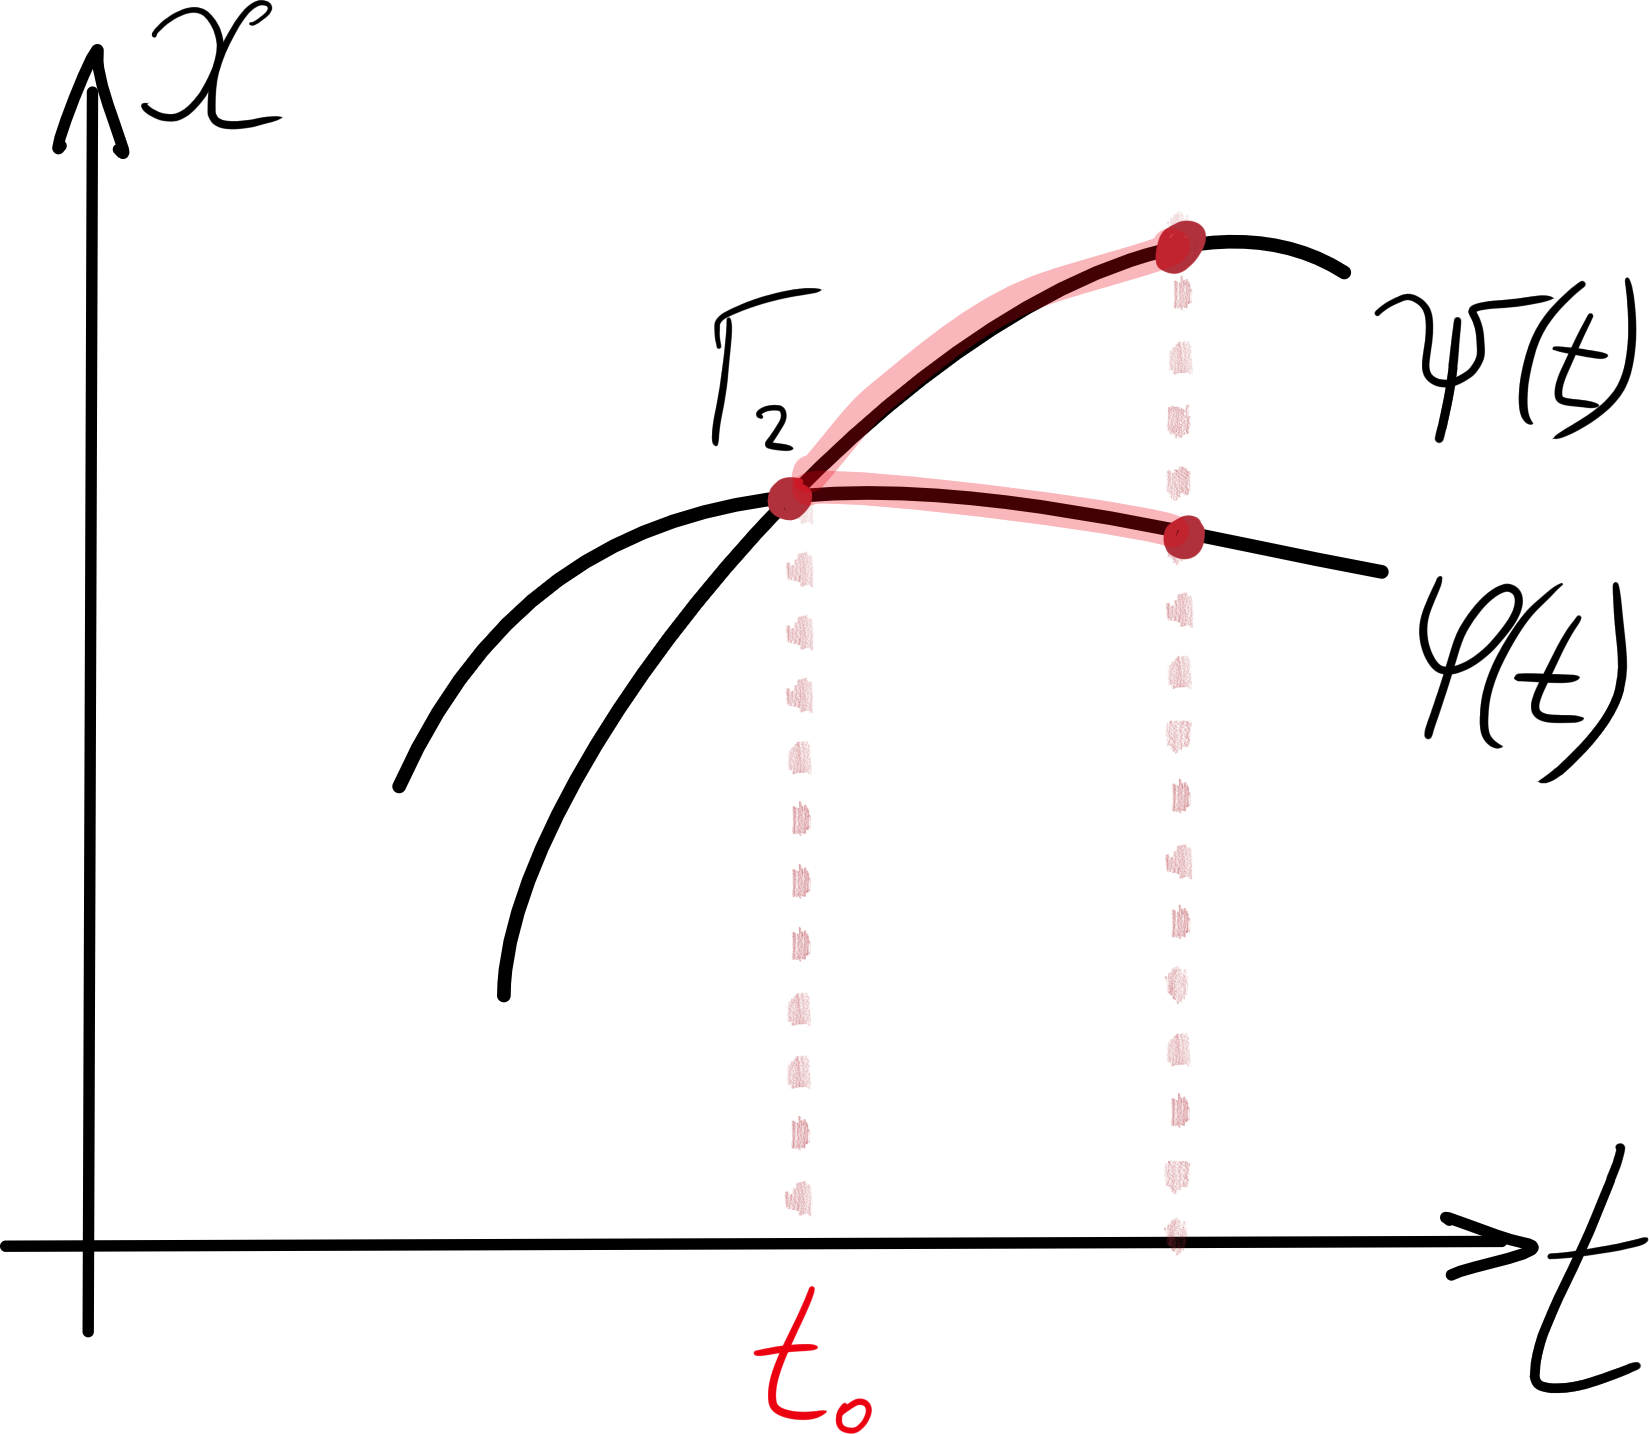
\includegraphics[width=4cm]{pics/9_1.png}
				    \centering
				\end{figure}
        \[\Gamma_j \text{ - замк., огр. } (j = 1, 2)\]
        \[\Gamma = \Gamma_1 \cup \Gamma_2 \text{ - замк., огр.}\]
        \[\Ra X \in \Lip_x(\Gamma)\]
        \[\exists L : \forall (t, \overline{x}), (t, \overline{\overline{x}}) \in \Gamma\]
        \[\abs{X(t, \overline{x}) - X(t, \overline{\overline{x}})} \leq L \abs{
        \overline{x} - \overline{\overline{x}}} \qq (\text{\#}))\]
        \[\begin{matrix}
            x = \varphi(t)\\
            x = \psi(t)
        \end{matrix} \text{ - реш. З.К. } (1)(2) \Ra
        \begin{matrix}
            \varphi(t) = x_0 + \int_{t_0}^t X(\tau, \varphi(\tau))d\tau\\
            \psi(t) = x_0 + \int_{t_0}^t X(\tau, \psi(\tau))d\tau
        \end{matrix}\]
        \[\forall  t \in <a, b> \Ra \text{ и } \forall t \in [t_0, \Theta]\]
        \[\abs{\varphi(t) - \psi(t)} \leq \int_{t_0}^t \abs{X(\tau, \varphi(\tau)) -
        X(\tau, \psi(\tau))} d\tau \os{(\text{\#})}{\leq}\]
        \[\leq L \int_{t_0}^t \abs{\varphi(\tau) - \psi(\tau)}d\tau \Ra
        \varphi(t) = \psi(t) \qq \forall t \in [t_0, \Theta]\]
        \[u(\tau) \leq L\int_{t_0}^t u(\tau)d\tau \qq  (\text{Л. Гронуолла } c = 1)\]
    \end{Proof}

    \section{Продолжение решений}
    \begin{Example}[1]
        \[\dot{x} = x^2 + 1 \qq \text{З.К.} (0, 0)\]
        \[\frac{dx}{x^2 + 1} = dt\]
        \[\arctg x = t  + c\]
        \[x = \tg t \q\text{ реш З.К, опред на } (-\frac{\pi}{2}, \frac{\pi}{2})\]
    \end{Example}

    \begin{Example}[2]
        \[\dot{x} = x^2 \qq (0, 1)\]
        \[\frac{dx}{x^2} = dt\]
        \[-\frac{1}{x} = t + c\]
        \[x = -\frac{1}{t + c}\]
        \[x = \frac{1}{1 - t}\]
        \begin{figure}[H]
				    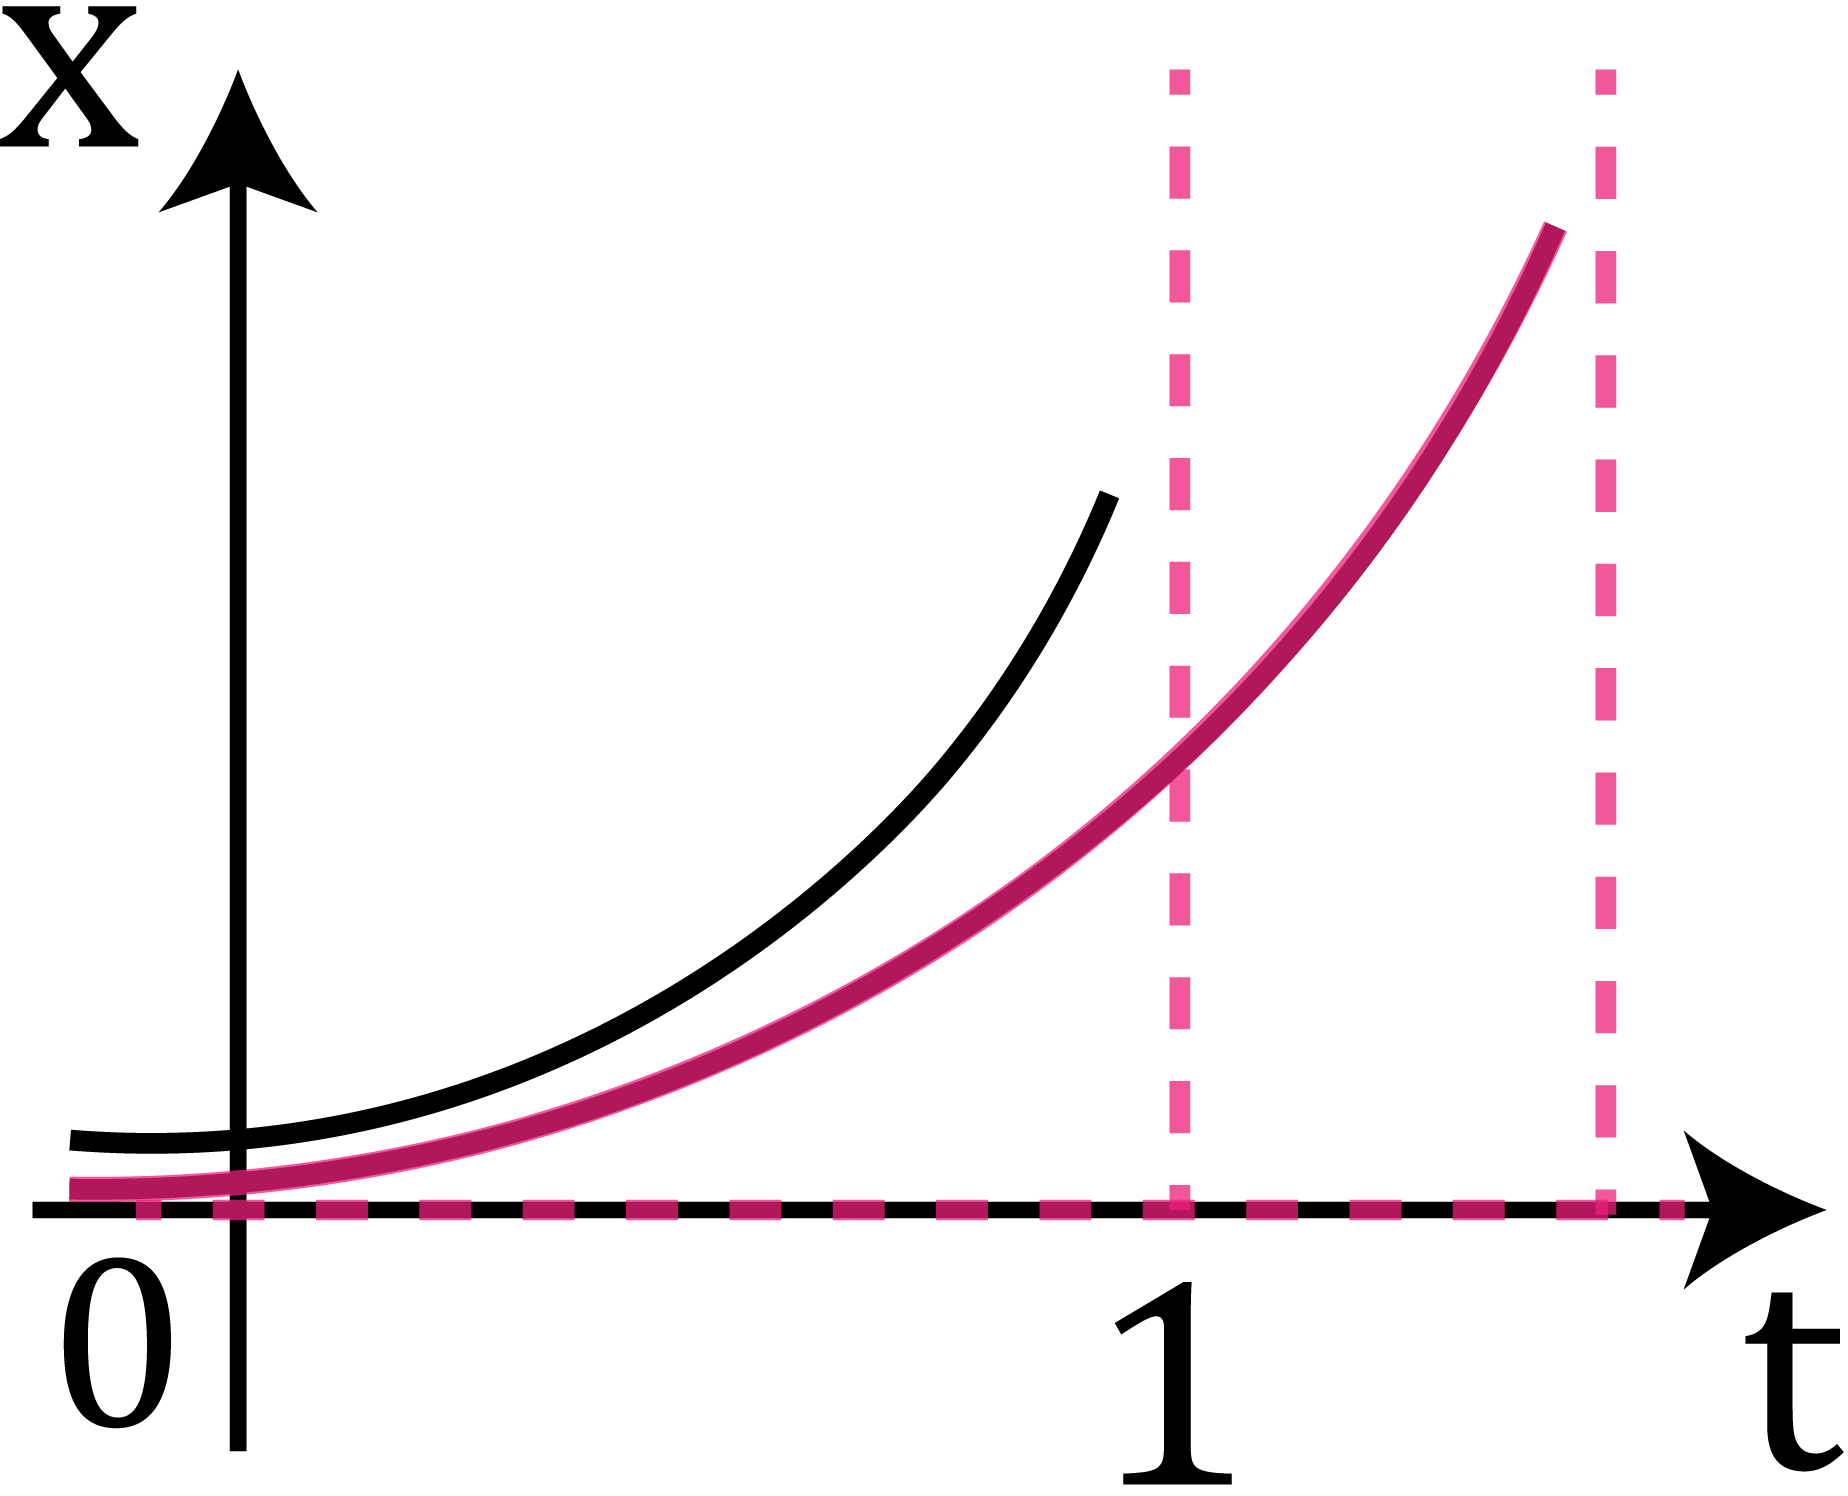
\includegraphics[width=4cm]{pics/9_2.png}
				    \centering
				\end{figure}
        \[t \in (-\infty, 1)\]
    \end{Example}

    \begin{Reminder}
        \[(1) \qq \dot{x} = X(t, x) \q \begin{cases}
            X \in C(G)\\
            X \in \Lip_x^{loc}(G), \qq \us{\text{обл}}{G} \subset \R^{n + 1}
        \end{cases}\]
        \[x = \varphi(t) \text{ - реш } (1), \q t \in (a, b)\]
    \end{Reminder}

    \begin{Definition}
        \[\text{реш } x = \varphi(t), \q t \in (a, b) \text{ продолжимо вправо за } b\]
        \[\text{если } \exists \text{ реш } (1) \q x = u(t)\text{, опред при } t \in
        (a, \overline{b}) \q \overline{b} > b, \]
        \[\text{такое, что } u(t) \equiv \varphi(t) \text{ на } (a, b)\]
        \[u(t) \text{ называется продолжением решения }\varphi(t)\]
        Аналогично определяется продолжимость решения влево за $a$
    \end{Definition}

    \begin{Theorem}
        \[\text{реш } x = \varphi(t) \q (t \in (a, b)) \text{ - продолжимо вправо за } b\]
        \[\rla \exists \lim_{t \to b-} \varphi(t) = \xi, \text{ и } (b, \xi) \in G\]
        \begin{figure}[H]
				    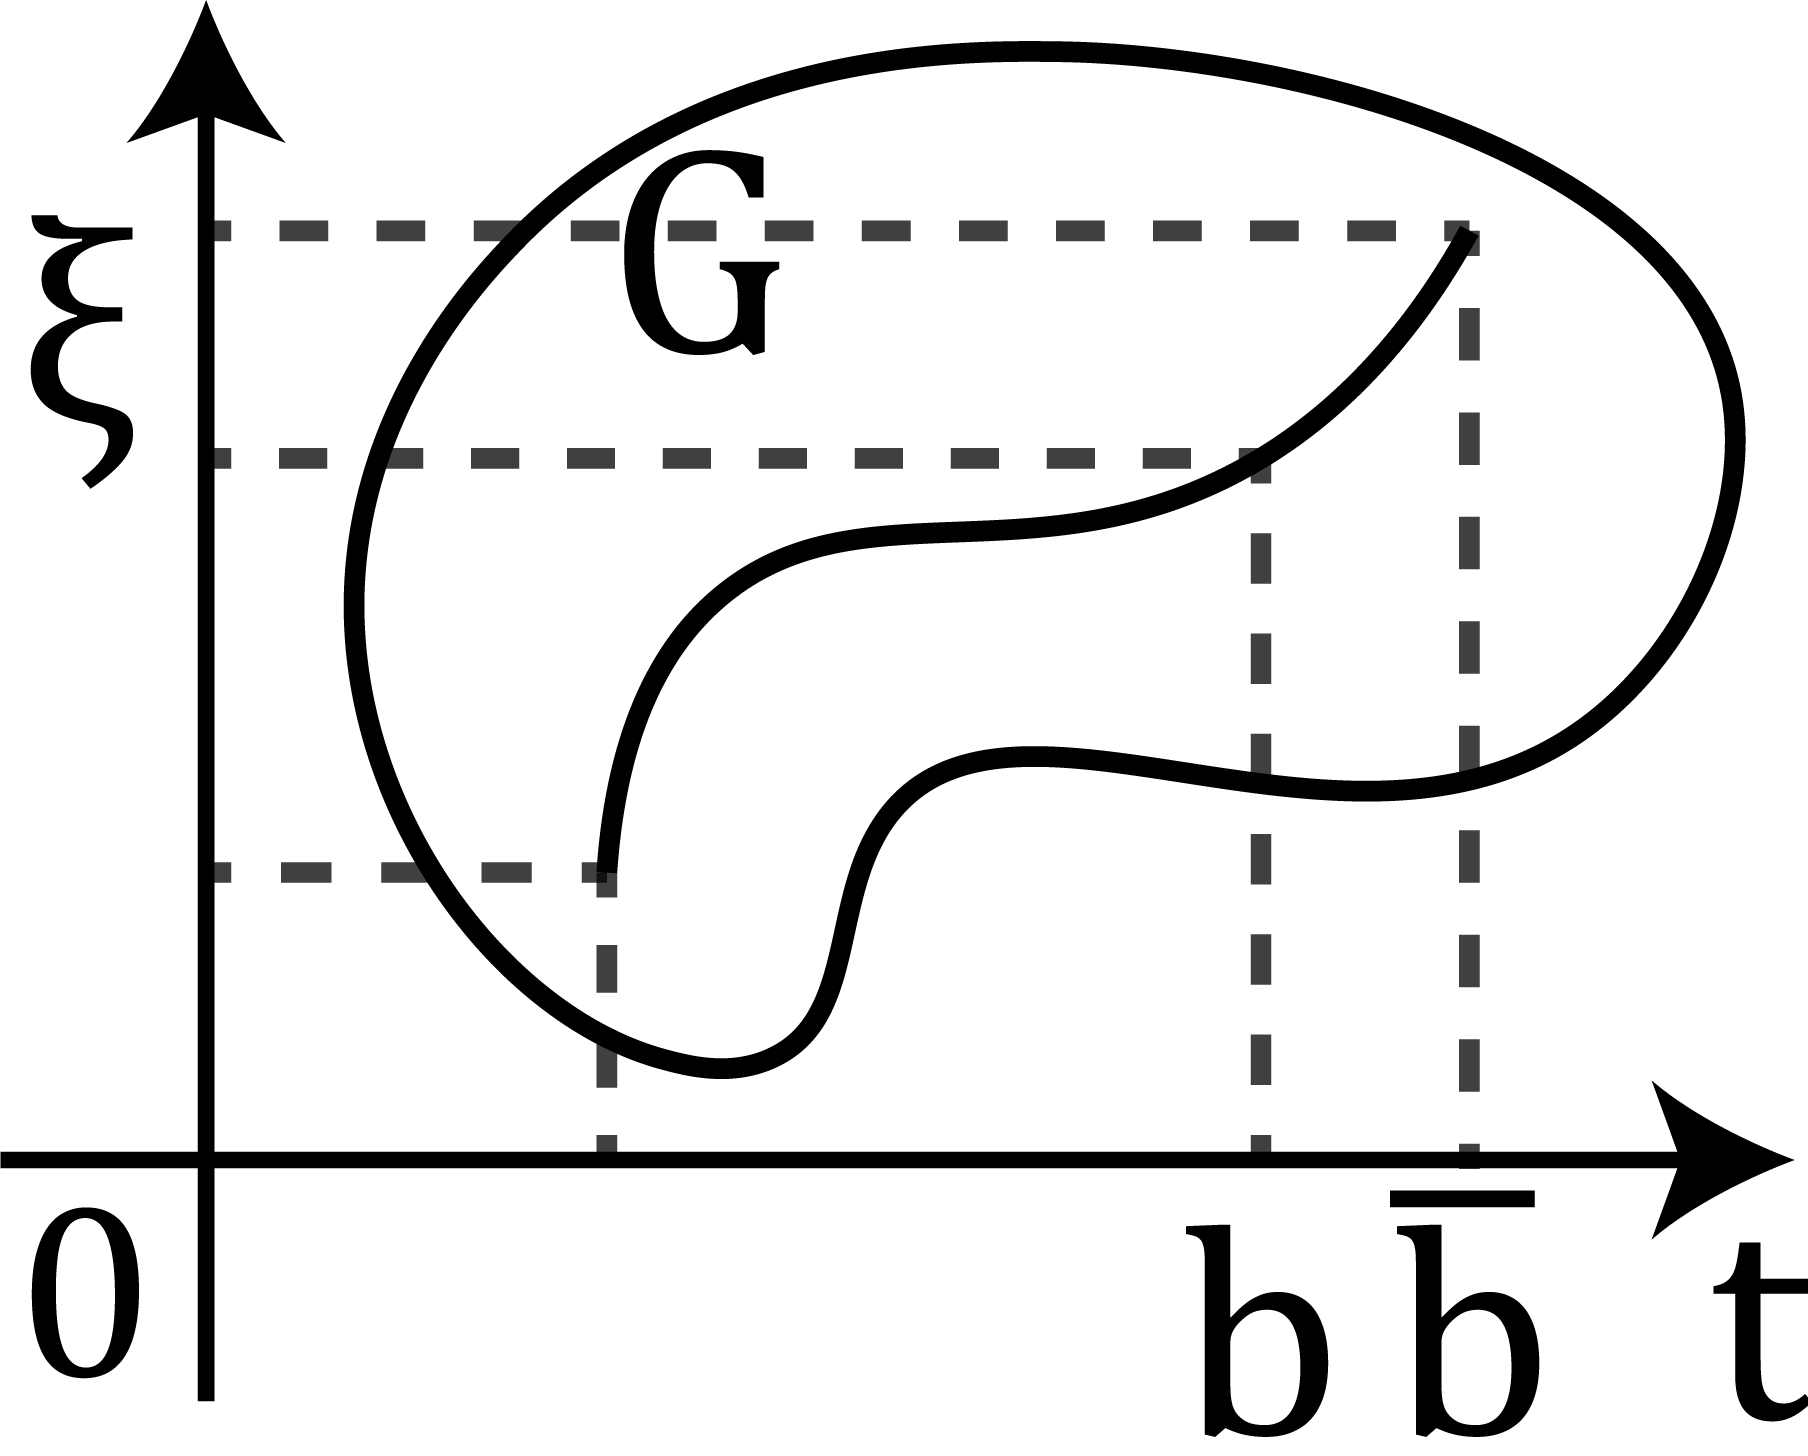
\includegraphics[width=4cm]{pics/9_3.png}
				    \centering
				\end{figure}
    \end{Theorem}

    \begin{Proof}
        \[\Ra) \q \exists \text{ реш } x = u(t) \qq t \in (a, \overline{b})\]
        \[\overline{b} > b, \q u(t) \equiv \varphi(t) \q \text{ на } (a, b)\]
        \[\Ra \lim_{t \to b-} \varphi(t) = \lim_{t \to b} u(t) = u(b) , \q
        (b, u(b)) \in G \]
        \[\La) \q \varphi(b) = \xi \text{ - по непр}\]
        \[\text{З.Коши } (b, \xi) \in G\]
        \[\exists h > 0 : \text{ на } [b - h, b + h] \text{ опред. решение } (1) \q
        x = w(t) : \q w(b) = \xi\]
        \[u(t) = \begin{cases}
            \varphi(t), & t \in (a, b]\\
            w(t), & t \in [b - h, b + h]
        \end{cases} \text{ - продолжение } \varphi(t)\]
        Определено корректно, т.к. $\varphi(t) \equiv w(t)$ на $[b - h, b]$ (почему?
        А потому что они решают одну задачу Коши)
    \end{Proof}

    \subsection{Максимальный промежуток задания решения}

    \begin{Theorem}[2]
        \[(1) \q \dot{x} = X(t, x)\]
        \[x = \varphi(t) \text{ - реш } (1), \q t \in (a, b) \q (\text{м.б }
        b = +\infty)\]
        \[\Ra \exists \beta \geq b : \exists  \text{ реш }
        (1)\ x = u(t) : \varphi(t) \equiv u(t) \text{ на } (a, b)\]
        \[\text{опред на } (a, \beta) \text{ и не продолжимо вправо за } \beta\]
    \end{Theorem}

    \begin{Proof}
        \[b = +\infty \Ra \beta = +\infty \Ra \text{ все д-но}\]
        \[\varphi(t) \text{ - не продолжимо вправо за } b \Ra \beta = b \Ra
        \text{ все доказано}\]
        Осталось: $b < +\infty$ и $\varphi(t) $ - продолжимо вправо за $b$
        \[B = \{\overline{b} : u(t) \text{ - продолжение } \varphi(t)
        \text{, опред на } (a, \overline{b})\}\]
        \[\overline{b} \in B \q  \text{ и } \q b < \Theta < \overline{b} \Ra \Theta \in B\]
        \begin{figure}[H]
				    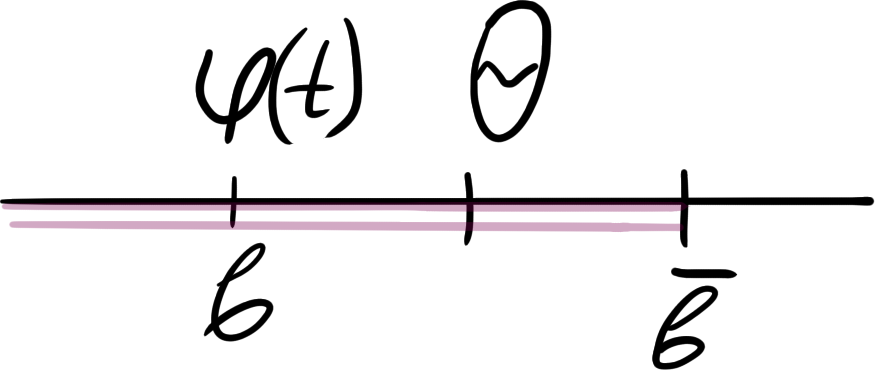
\includegraphics[width=4cm]{pics/9_4.png}
				    \centering
				\end{figure}
        \[\overline{b}_1, \overline{b}_2 \in B, \q \overline{b}_1 < \overline{b}_2 \qq
        u_{\overline{b}_1}, u_{\overline{b}_2} \text{ - соотв. прод-я } \varphi(t)  \]
        \[\Ra u_{\overline{b}_1} \equiv u_{\overline{b}_2} \text{ на } (a,
        \overline{b}_1)  \]
        \[\beta = \sup B\]
        \[\text{если } \beta = +\infty \Ra \text{ все доказано}\]
        \[\text{если } \beta < +\infty\]
        \[\exists  \text{ продолжение } \varphi(t) \text{ на } (a, \beta),
        \text{т.е. } u_{\beta}(t) \text{ - реш } (1) \text{ опред на } (a, \beta) \]
        \[(u_{\beta}(t) \equiv \varphi(t) \text{ на } (a, b))\]
        \[t \in [b, \beta) \Ra  \exists \overline{b} \in B : \text{ опред-но }
        u_{\overline{b}}(t) \]
        \begin{figure}[H]
				    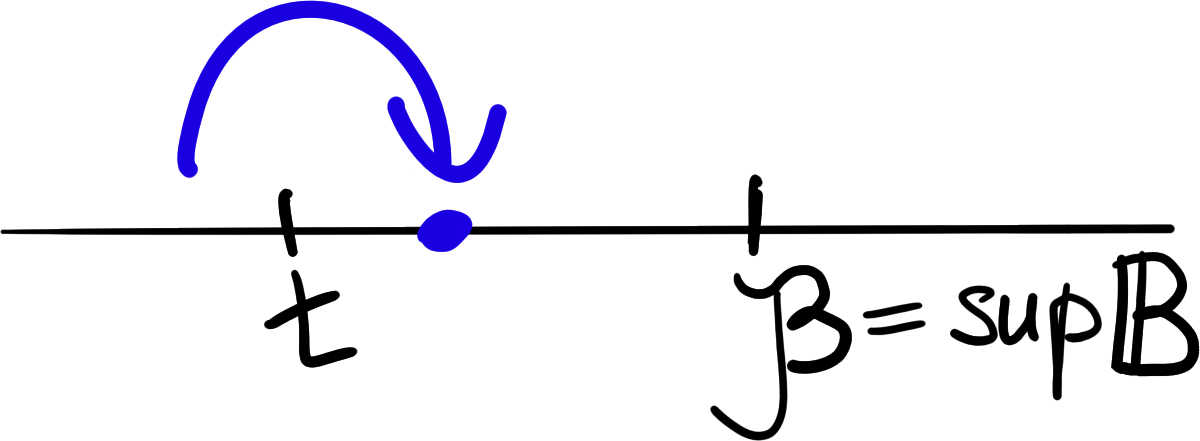
\includegraphics[width=4cm]{pics/9_5.png}
				    \centering
				\end{figure}
        Докажем, что $u_{\beta}(t)$ не продолжимо ща $\beta$ вправо
        \[\letus \exists \widetilde{\beta} > \beta : U_{\beta}(t) \text{ - продолжимо до }
        \widetilde{\beta} \Ra \widetilde{\beta} \in B\]
        Противоречит супремуму\\
    \end{Proof}

    \begin{Theorem}[2']
        \[\text{Аналогично влево}\]
    \end{Theorem}

    \begin{Consequence}
        \[\forall  \text{ реш }(1) \q x = \varphi(t), \text{ опред на } (a, b) \]
        \[\exists  \begin{cases}
            \alpha \leq a\\
            \beta \geq b
        \end{cases} : \q \exists  \text{ реш } (1) \q x = w(t) : \q w(t) \equiv
        \varphi(t) \text{ на } (a, b)\]
        \[w(t) \text{ опред на } (\alpha, \beta) \text{ и не продолжимо ни вправо
        за $\beta$ ни влево за } \alpha \]
    \end{Consequence}

    \begin{Proof}
        \[w(t) = \begin{cases}
            u(t), & t \in (a, \beta) \qq (\beta \text{ из } T_2)\\
            v(t), & t \in (\alpha, b) \qq (\alpha \text{ из } T_2')
        \end{cases}\]
        \[(u(t) \equiv v(t) \equiv \varphi(t) \text{ на } (a, b))\]
    \end{Proof}

    \begin{Definition}
        \[\text{промежуток } (\alpha, \beta) \text{ называется максимальным
        промежутком задания}\]
    \end{Definition}

    Теперь мы рассматриваем решения с макс. промежутком задания.
\end{lect}
\end{document}
